\documentclass[border=0.8ex,svgnames,tikz]{standalone}
\usepackage{amsmath,mathtools}
\usepackage{fontspec}
\setmainfont{Source Serif 4}
\setsansfont{Source Sans 3}
\setmonofont{Source Code Pro}
\usetikzlibrary{chains}
\begin{document}
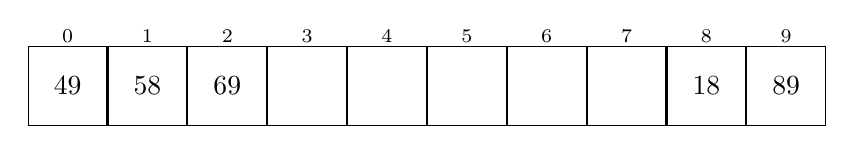
\begin{tikzpicture}[every node/.style={minimum height=1cm,minimum width=1cm}]
  \begin{scope}[
    node distance=0,
    xnode/.append style={draw,on chain},
    index node/.append style={draw=none,inner sep=0ex,minimum
      height=1.5ex,font=\scriptsize},
    start chain=going right,
    ]
    \foreach \i in {0,...,9}{
      \node[xnode](node\i){};
      \node[index node,above=of node\i](idx\i){\i};
      \chainin(node\i);
    };
  \end{scope}
  \node at(node0) {49};
  \node at(node1) {58};
  \node at(node2) {69};
  \node at(node8) {18};
  \node at(node9) {89};
\end{tikzpicture}
\end{document}
